\section{Tests and Results}
\par
\begin{figure}[H]
\centering
  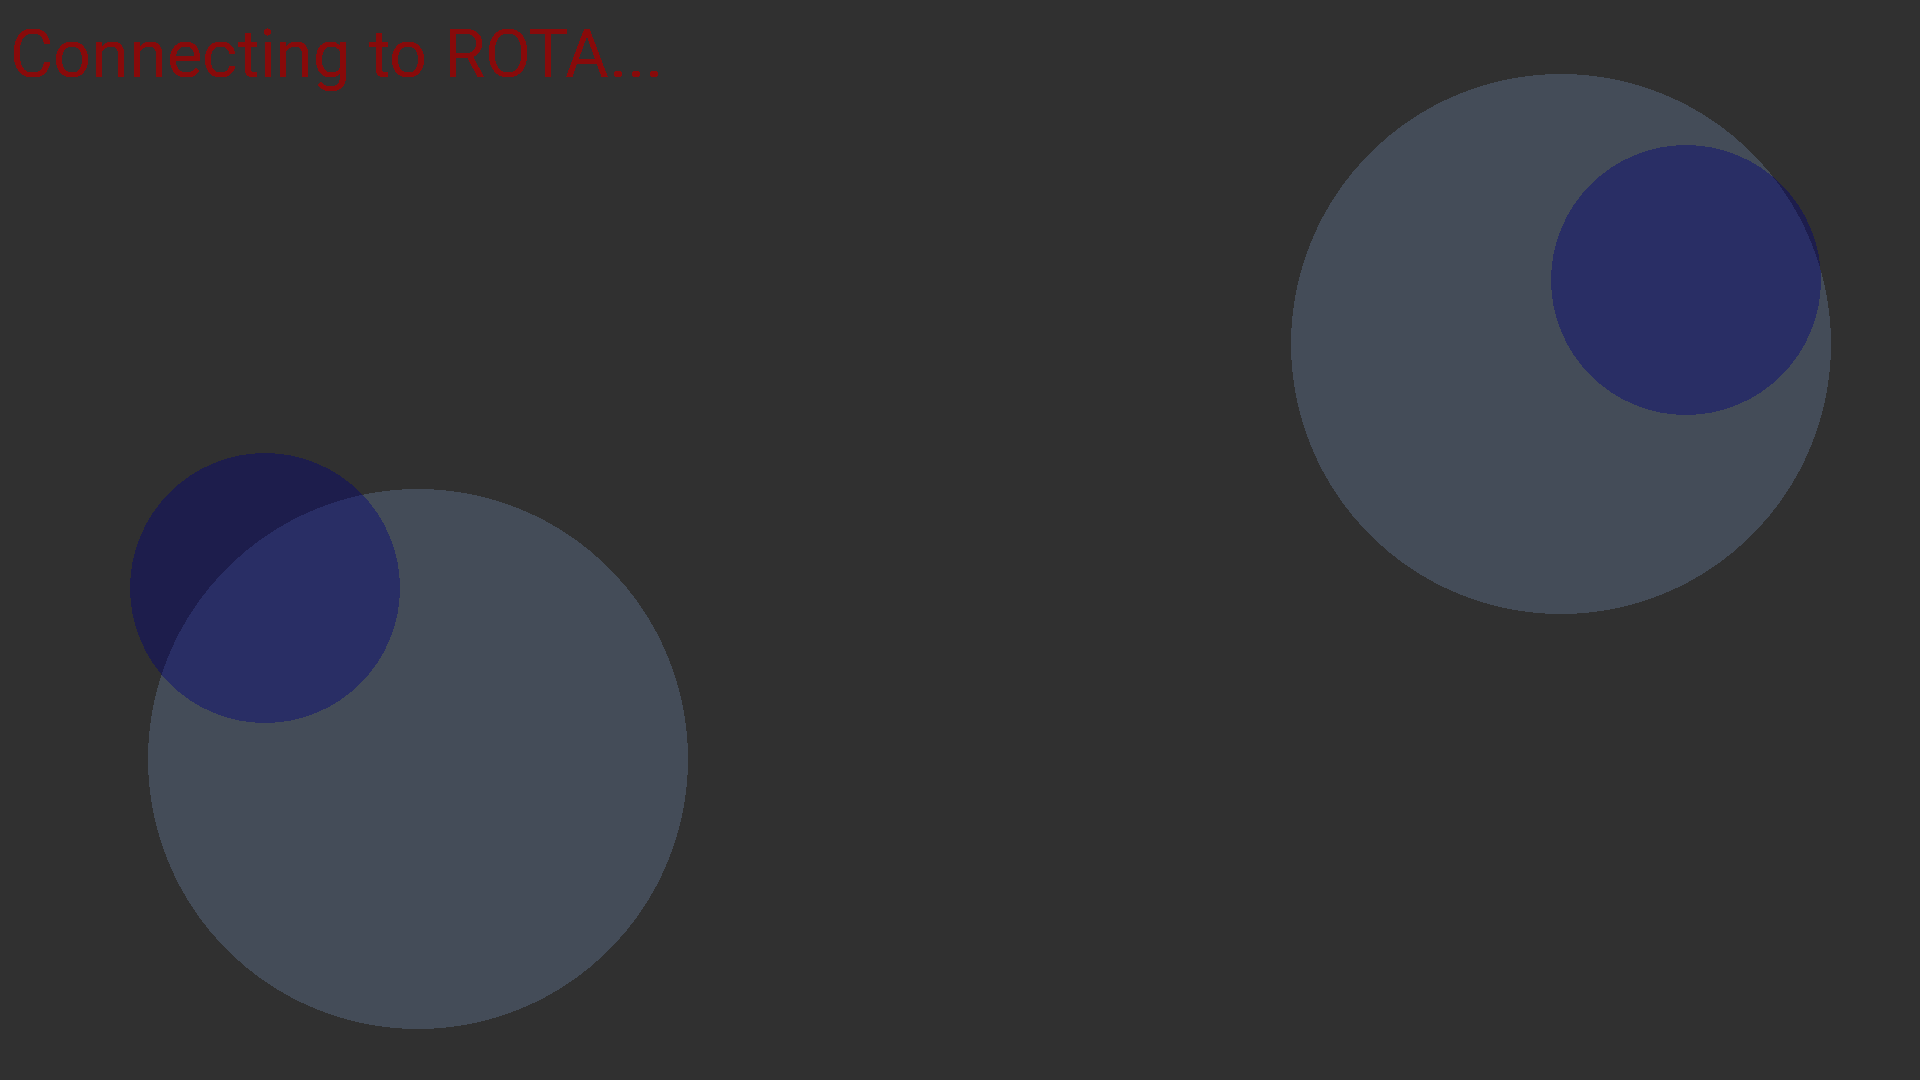
\includegraphics[width=0.6\textwidth]{sections/testRes/app1}
    \caption{A photo showing the joysticks in the app.}
\end{figure}
\begin{figure}[H]
\centering
  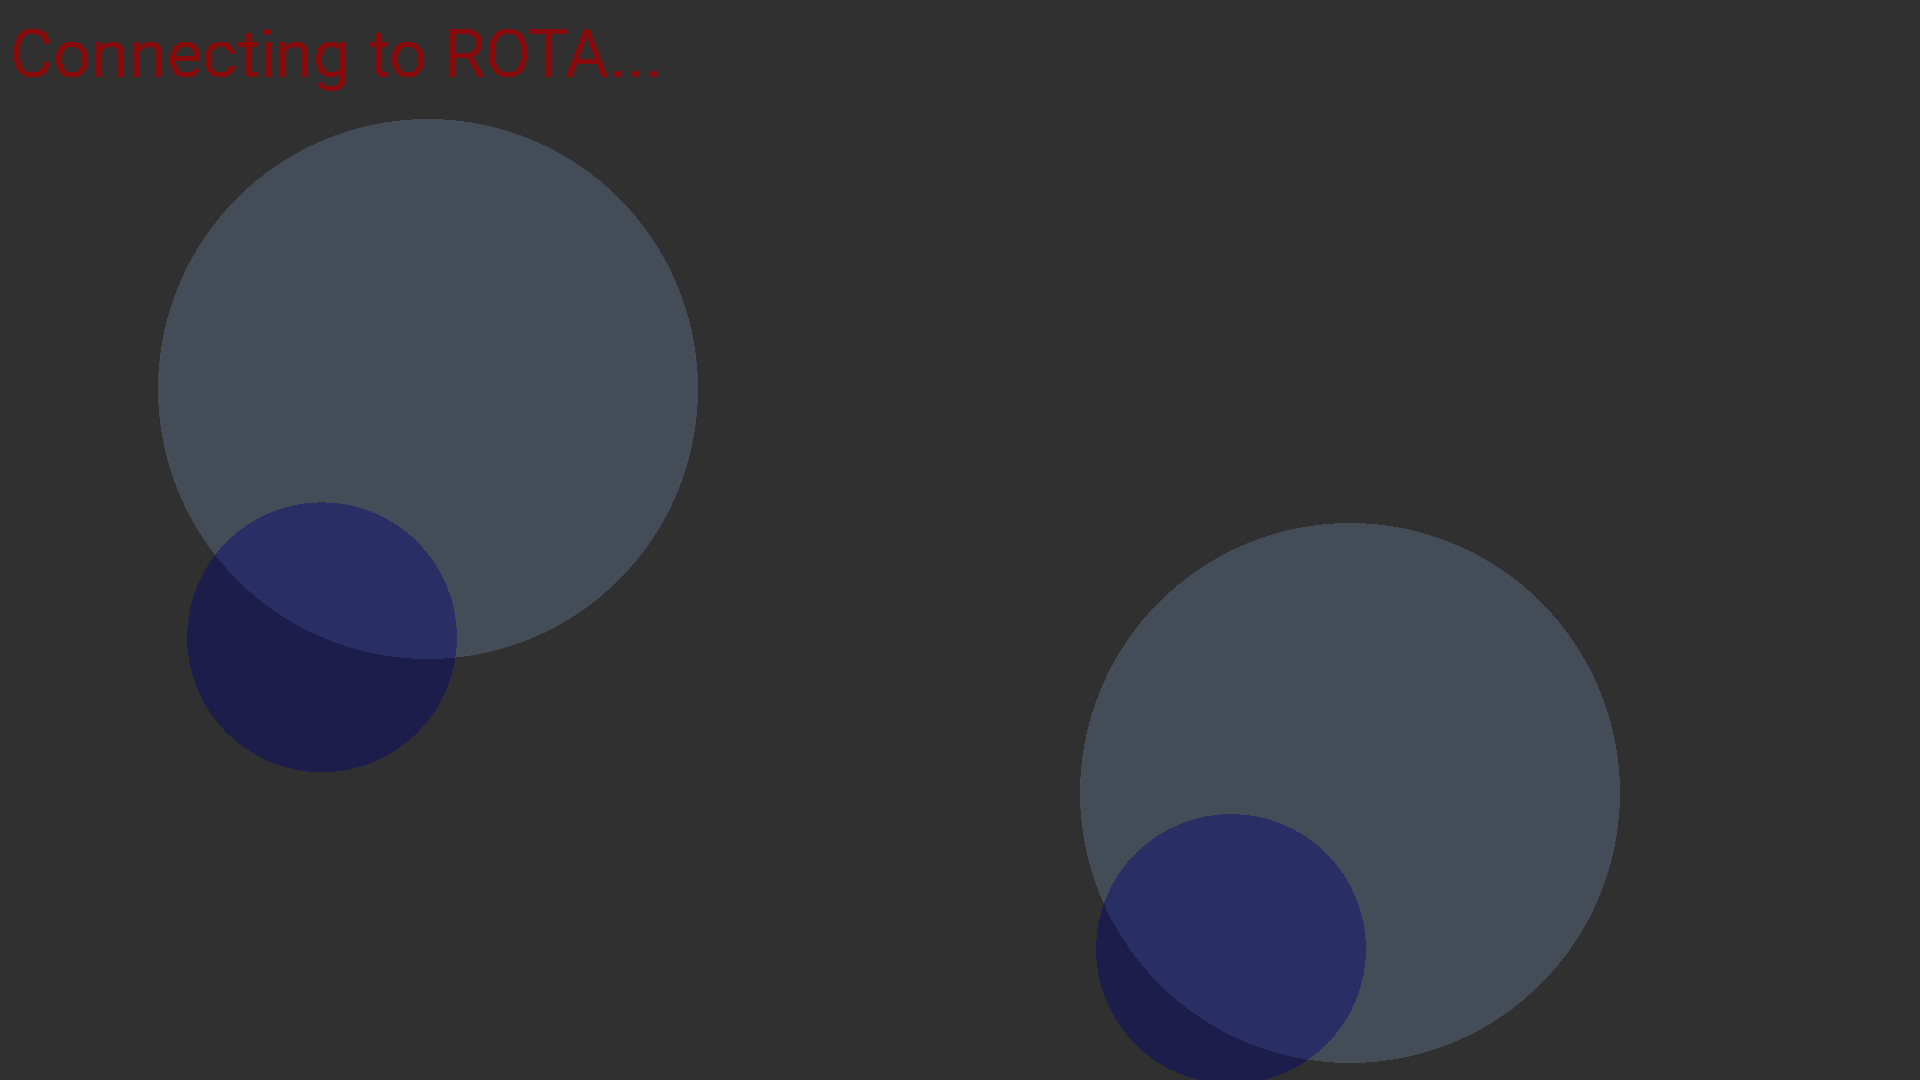
\includegraphics[width=0.6\textwidth]{sections/testRes/app2}
    \caption{Another photo showing the joysticks in the app. This shows how the joysticks will move when the user touches the screen.}
\end{figure}
\begin{figure}[H]
\centering
  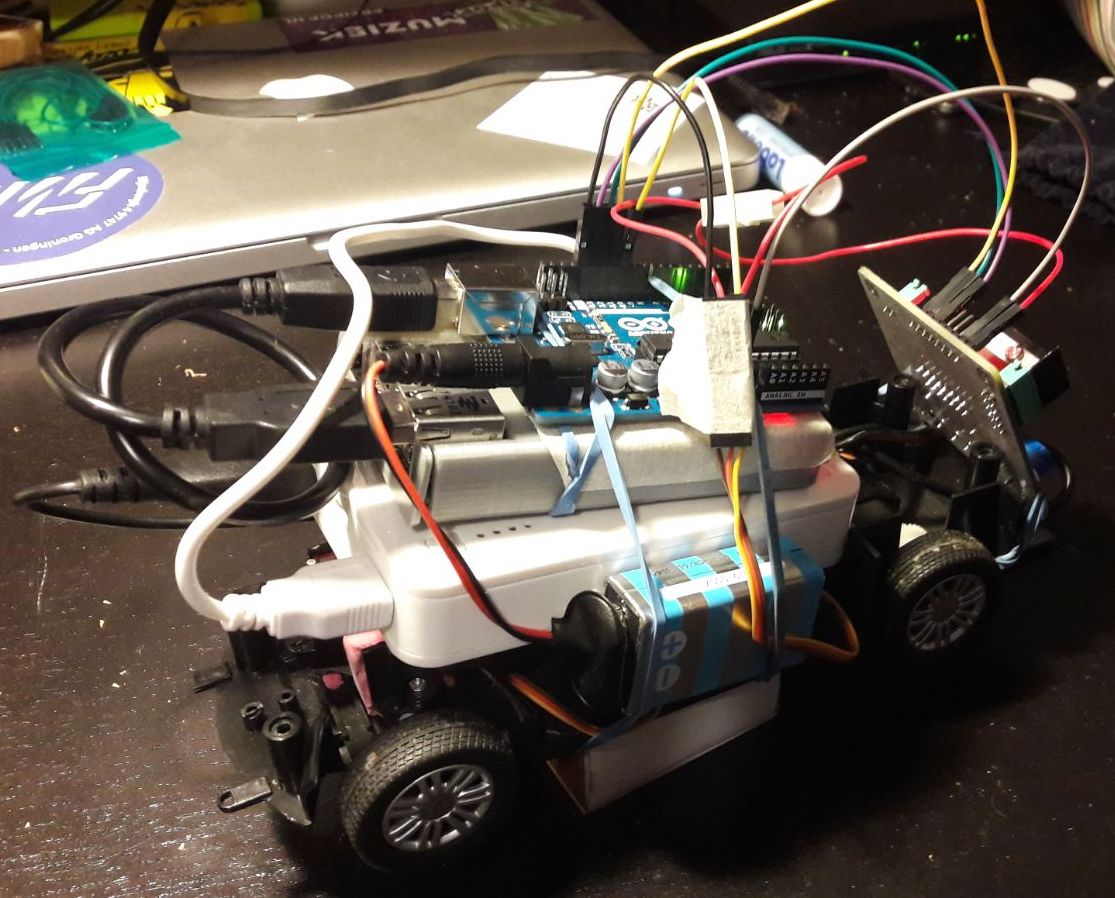
\includegraphics[width=0.6\textwidth]{sections/testRes/left}
    \caption{A view of the left side of the finished car.}
\end{figure}
\begin{figure}[H]
\centering
  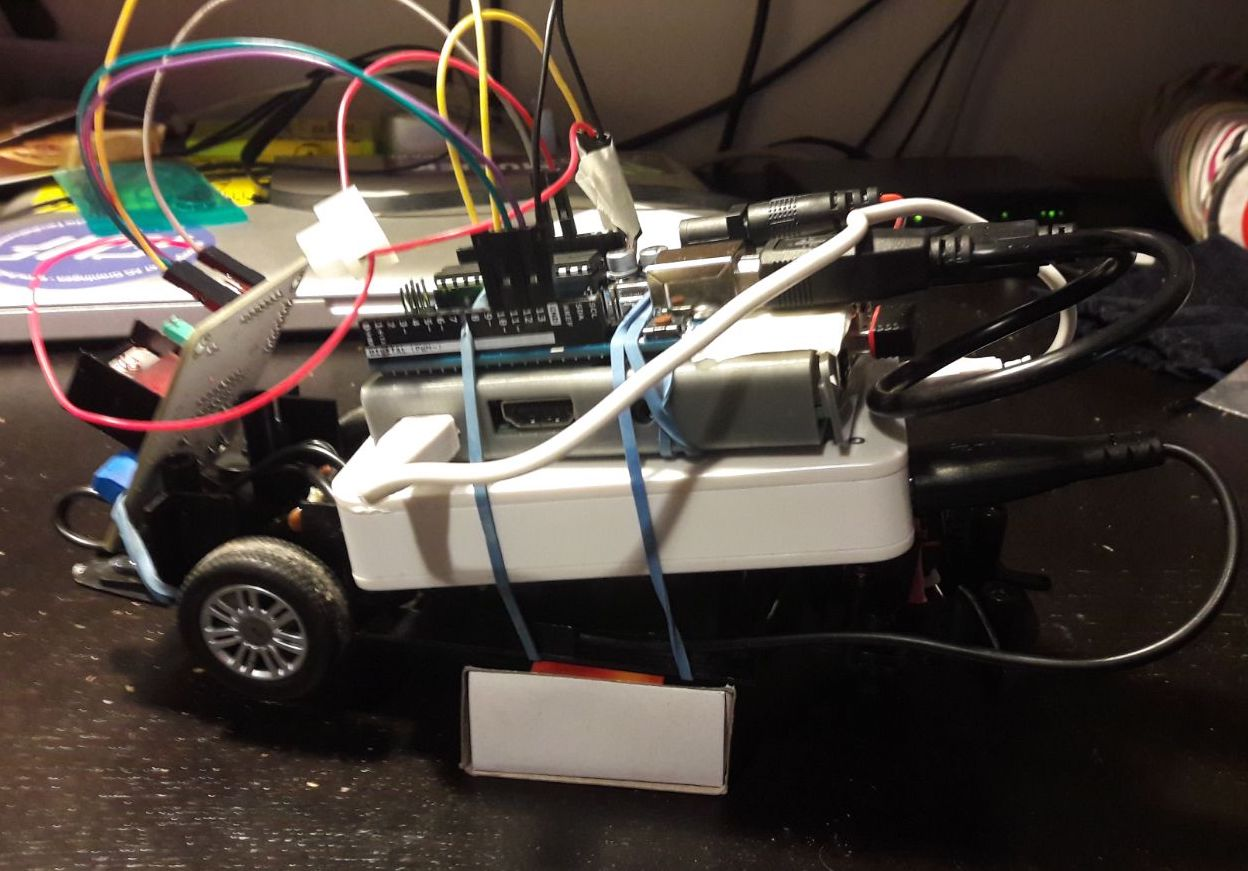
\includegraphics[width=0.6\textwidth]{sections/testRes/right}
    \caption{A view of the right side of the finished car. You may notice the missing front wheel that was being repaired at the time of this photograph.}
\end{figure}
\begin{figure}[H]
\centering
  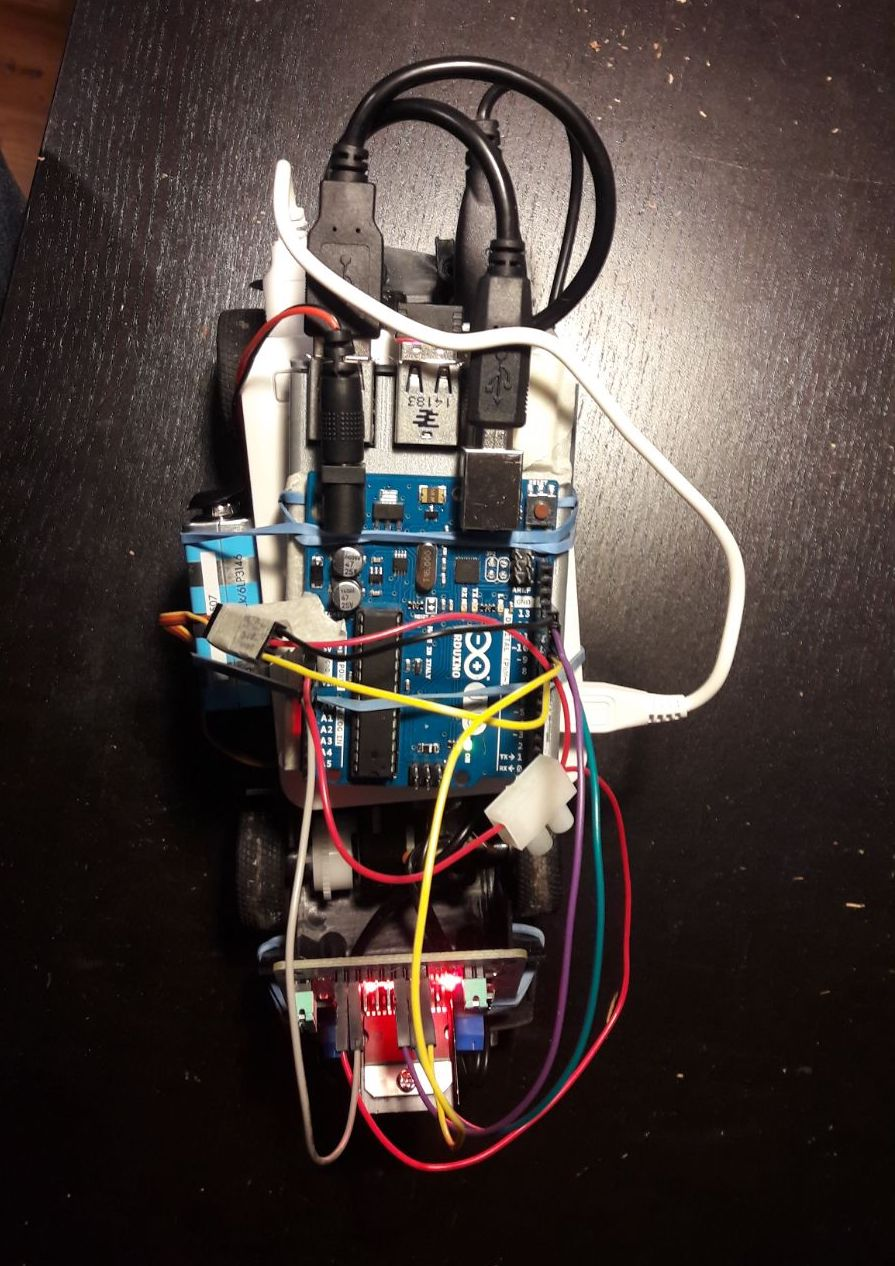
\includegraphics[width=0.6\textwidth]{sections/testRes/top}
    \caption{A view of the top of the finished car.}
\end{figure}
